\section{Verifying a Simplified Eio Scheduler with Promises}
\label{sec:scheduler}

\todo{Mention that all code examples are an OCaml rendering of the verified \hazel{} code, based on but not equal to the Eio code}

Cooperative concurrency schedulers for user-level threads (i.e. \emph{fibers}) are commonly treated in the literature
on effect handlers~\cite{dolan2018concurrent,leijen2017structured,de2021separation} to because they are a good example for the usefulness
of manipulating delimited continuations with effect handlers.
Generally, the architecture contains an effect handler as the scheduler and fibers are normal functions which perform effects to yield execution.
This is because performing an effect causes execution to jump to the enclosing effect handler (i.e. the scheduler), providing it with the rest of the fiber's computation in the form of a delimited continuation.
The scheduler keeps track of a collection of these continuations and by invoking one of them the next fiber is scheduled.
This approach is also used in Eio.

We can therefore use the simple cooperative concurrency scheduler case study from the dissertation of de Vilhena~\cite{de2022proof} as a starting point for our verification work.
In the following section we first discuss the implementation of our simplified model of Eio in more detail.
Using this implementation we give an intuition about what specifications the functions should satisfy and what kind of logical state is needed to prove these specifications.
Based on this intuition we will then build a formalization in section~\ref{sec:sched-spec}.
% But some key differences in the implementation of Eio allow simplifications of the logical state that we use in our proofs. 

\subsection{Implementation}
\label{sec:sched-impl}

Let us first get an idea of how different components of the core Eio fiber abstraction interact by looking at their types.
\ocamlin{Scheduler.run}\footnote{The scheduler's result is optional because the main fiber might deadlock.} is the main entry point to Eio.
It runs a scheduler and is provided a function which represents the first fiber to be executed.
A scheduler runs the main fiber and all forked-off fibers in a single thread.
However, a fiber can also spawn new schedulers in separate threads to run other fibers in parallel as detailed in appendix~\ref{sec:apdx-mt}.
The \ocamlin{Fiber.fork_promise} function is used to spawn fibers in the current scheduler.
The function returns a promise holding the eventual return value of the new fiber.
The promise is thread-safe so that it can be shared with fibers running in different threads.
The \ocamlin{Promise.await} function can be used by any fiber to wait until the value of a promise is available.
Common problems like deadlocks are not prevented in any way and are the responsibility of the programmer.
% The function sends the fiber to the scheduler by performing an effect, so it must always be called from a fiber itself.


\begin{minted}{ocaml}
  (* Basic interface of the Eio library. *)
  Scheduler.run : (unit -> 'a) -> 'a option
  Fiber.fork_promise : (unit -> 'a) -> 'a Promise.t
  Promise.await : 'a Promise.t -> 'a
\end{minted}

\subsubsection{\ocamlin{Scheduler.run}}
\label{sec:sched-impl-run}

\begin{figure}[ht]
  \begin{minted}[escapeinside=@@]{ocaml}
effect Fork : (unit -> 'a) -> unit
type 'a waker : 'a -> unit
effect Suspend : ('a waker -> unit) -> 'a

let run (main : unit -> 'a) : 'a option =
  let run_queue = Lf_queue.create () in @\label{ln:run6}@
  let next () =
    match Lf_queue.pop run_queue with
    | None -> ()
    | Some cont -> cont () 
  in
  let rec execute fiber =
    match fiber () with
    | () -> next ()
    | @\texttt{\textbf{effect}}@ (Fork fiber) k ->
        Lf_queue.push run_queue (fun () -> invoke k ());
        execute fiber
    | @\texttt{\textbf{effect}}@ (Suspend register) k =>
        let waker = fun v -> Lf_queue.push run_queue (fun () -> invoke k v) in
        register waker;
        next ()
  in
  let result = ref None in
  execute (fun () -> result := main ());
  !result
  \end{minted}
  \caption{Implementation of \ocamlin{Scheduler.run}}
  \label{fig:sched-impl-run}
\end{figure}

As mentioned above this is the main entry point to the Eio library and its code is shown in figure~\ref{fig:sched-impl-run}.
It sets up the scheduler environment and runs the main fiber that is passed as an argument.

The \ocamlin{run_queue} (line~\ref{ln:run6}) contains closures that will immediately invoke the continuation of an effect.
This represents ready fibers which can continue execution from the point where they performed an effect.
The \ocamlin{next} function (line 7) pops one fiber (i.e. function) from the \ocamlin{run_queue} and executes it.
If no more ready fibers remain -- either because all fibers terminated or there is a deadlock -- the \ocamlin{next} function returns and the scheduler exits.

The inner \ocamlin{execute} function (line 12) is called once on each fiber to evaluate it and handle any performed effects.
\subsubsection*{Value Case}
The non-effect case of the \ocamlin{match} (line 14) only runs the next fiber because Eio adopts the convention that all fibers return a unit value and their real return value is handled out of band.
\begin{itemize}
  \item The main fiber is wrapped in a closure that saves its return value in a reference (line 24) that is read when the scheduler exits (line 25).
  \item All other fibers are forked using \ocamlin{Fiber.fork_promise}, which wraps them in a closure that saves their return value in a promise.
\end{itemize}

This emphasizes the fact that an Eio scheduler is only used for running fibers.
The interaction between fibers waiting for values of other fibers is handled separately by promises.

\subsubsection*{\efork{} Case}
Handling a \efork{} effect (line 15) is simple because it only carries a new \ocamlin{fiber} to be executed, so the handler recursively calls the \ocamlin{execute} function (line 17) to execute it immediately.
The execution of the original fiber is paused due to performing an effect and its continuation \ocamlin{k} is placed in the run queue so that it can be scheduled again (line 16).
This prioritizes the execution of a new fiber and is a design decision by Eio.
It would be equally valid to place the \ocamlin{fiber} argument in the run queue instead.

\subsubsection*{\esuspend{} Case}
Handling a \esuspend{} effect (line 18) may look complicated at first due to the higher-order \ocamlin{register} function.
This effect is used by fibers to suspend execution until a condition is met.
The fiber defines this condition by constructing a \ocamlin{register} function which in turn receives a wake-up capability by the scheduler in the form of a \ocamlin{waker} function.
The key point is that as long as the continuation \ocamlin{k} is not invoked, the fiber will not continue execution.
So the \ocamlin{waker} function "wakes up" a fiber by placing its continuation \ocamlin{k} into the run queue (line 19).
The \ocamlin{register} function is called by the scheduler right after the fiber suspends execution (line 20) and is responsible for installing \ocamlin{waker} as a callback at a suitable place (or even call it directly).
For example, to implement promises, the \ocamlin{waker} function is installed in a data structure that will call \ocamlin{waker} after the promise is fulfilled.

Note that the \ocamlin{waker} function's argument \ocamlin{v} has a \emph{locally abstract type}, which is a typical pattern in effect handlers.
From the point of view of the fiber, the polymorphic type \ocamlin{'a} of the \esuspend{} effect is instantiated depending on how the effect's return value is used.
But the scheduler does not get any information about this so the argument type of the continuation \ocamlin{k} and the \ocamlin{waker} function is abstract.

Waking up must be possible across thread boundaries, which is why the \ocamlin{run_queue} in the scheduler is a thread-safe queue.
For the verification we assume the specification of a suitable \ocamlin{Lf_queue} module that supports thread-safe push and pop operations, which exists in Eio under the same name.

% <!-- In our simplified model of Eio, the `Suspend` effect is only performed in the implementation of `Promise.await` which registers the `waker` callback to be called when the promise is fulfilled. -->

\subsubsection{\ocamlin{Fiber.fork_promise}}
\label{sec:sched-impl-fork}

\begin{figure}[ht]
  \begin{minted}{ocaml}
(* promise.ml *)
type 'a t = Done of 'a | Waiting of Broadcast.t

let create () : 'a t = 
  let bcst = Broadcast.create () in
  Atomic.create (Waiting bcst)

let fulfill p result =
  match Atomic.get p with
  | Done _ -> error "impossible"
  | Waiting bcst ->
      Atomic.set p (Done result);
      Broadcast.signal_all bcst
  
(* fiber.ml *)
let fork_promise (f : unit -> 'a) : 'a Promise.t =
  let p = Promise.create () in
  let fiber = fun () ->
    let result = f () in
    Promise.fulfill p result
  in
  perform (Fork fiber) 
  p
  \end{minted}
  \caption{Subset of the interface of the \ocamlin{Promise} module \& implementation of \ocamlin{Fiber.fork_promise}}
  \label{fig:sched-impl-fork}
\end{figure}

This function is the basic way to fork a new fiber in Eio and the only one we model in our development.
The code is presented in figure~\ref{fig:sched-impl-fork}.
It creates a promise (line 17) and spawns the provided function as a new fiber using the \efork{} effect (line 22).
Promises are always created in a \ocamlin{Waiting} (or unfulfilled) state and calling \ocamlin{Promise.fulfill} will move it to the \ocamlin{Done} state, at which point the final value can be retrieved.
The meaning of the \ocamlin{Broadcast.t} is explained in the next section.

When \ocamlin{f} is reduced to a value \ocamlin{result}, \ocamlin{Fiber.fork_promise} then fulfills the promise with that value (line 20), which will signal all fibers waiting for that result to wake up (line 13).
The major difference with respect to the implementation of de Vilhena is that promises in Eio are entirely handled by the fiber, and not in the effect handler code of the scheduler.
This achieves a better separation of concerns and simplifies the logical state needed for the proof.

\subsubsection{\ocamlin{Promise.await}}
\label{sec:sched-impl-await}

\begin{figure}[ht]
  \begin{minted}{ocaml}
let make_register (p: 'a t) (bcst: Broadcast.t) : (unit waker -> unit) = 
  fun waker ->
    let register_result = Broadcast.register bcst waker in
    match register_result with
    | None -> ()
    | Some register_handle ->
      match Atomic.get p with
      | Done result ->  
          if Broadcast.try_unregister register_handle
          then waker ()
          else ()
      | Waiting _ -> ()

let await (p: 'a t) : 'a = 
  match Atomic.get p with
  | Done result -> result
  | Waiting bcst ->
    let register = make_register p bcst
    perform (Suspend register);
    match Atomic.get p with
    | Done result -> result 
    | Waiting _ -> error "impossible"
  \end{minted}
  \caption{Implementation of \ocamlin{Promise.await}}
  \label{fig:sched-impl-await}
\end{figure}

This is the most complex looking function in our development which is partly due to the \esuspend{} effect and also due to the use of \emph{broadcast} functions.
Its code is presented in figure~\ref{fig:sched-impl-await}.
The purpose of \ocamlin{Promise.await p} is to suspend execution of the calling fiber until \ocamlin{p} is fulfilled with a value and then return this value.
The "suspend execution" part is handled by performing a \esuspend{} effect.
Then, the "until \ocamlin{p} is fulfilled" part is implemented by using a \emph{broadcast} data structure.

In Eio, a \emph{broadcast} is an implementation of a signalling mechanism used for similar purposes as condition variables in various languages.
The major difference is that callers do not directly suspend execution if the condition is not met, but supply a callback that will be called when the condition is signalled.

In figure~\ref{fig:sched-impl-broadcast} we show the public API of the \ocamlin{Broadcast} module.
The \ocamlin{Broadcast.register} function attempts to register a given callback with the data structure while \ocamlin{Broadcast.signal_all} calls all registered callbacks.
For \ocamlin{Broadcast.register}, a return value of \ocamlin{Called} means that it already called the supplied callback because the function detected the signal while it was running.
Otherwise, a return value of \ocamlin{Registered register_handle} means that the callback was registered but the signal might have been already sent but missed.
It is the responsibility of the caller to check if the signal was already sent and if it was, to then cancel the registration again
This is done by calling the \ocamlin{Broadcast.try_unregister} function on the \ocamlin{register_handle}, which returns a boolean indicating the cancellation status.
If the cancellation was successful, the previously registered callback will not be called when \ocamlin{Broadcast.signal_all} is executed.
The implementation and specification of the functions will be expanded upon in section~\ref{sec:broadcast}, for now we just explain their usage in the context of \ocamlin{Promise.await}.

\begin{figure}[ht]
  \begin{minted}{ocaml}
type t
type signal = unit -> unit
type register_result = Called | Registered of register_handle
type register_handle

val create : unit -> t
val register : t -> signal -> register_result
val try_unregister : register_handle -> bool
val signal_all : t -> unit
  \end{minted}
  \caption{Interface of the \ocamlin{Broadcast} module.}
  \label{fig:sched-impl-broadcast}
\end{figure}

In the \ocamlin{Promise.await} function if the promise is not fulfilled initially (figure~\ref{fig:sched-impl-await} line 23) then the fiber should wait until that is the case, so it performs a \esuspend{} effect (line 25).
The \ocamlin{register} function passed to the effect will register the \ocamlin{waker} function using \ocamlin{Broadcast.register} (line 9).
When at some point the \ocamlin{Broadcast.signal_all} function is called -- this happens in \ocamlin{Fiber.fork_promise} -- all registered \ocamlin{waker}s will be called in turn.
Recall that calling a \ocamlin{waker} function will enqueue the fiber that performed the \esuspend{} effect in the scheduler's run queue so that it can continue execution.

In the default case the following simplified chain of events happens:
\begin{enumerate}
  \item The fiber suspends execution at the point of evaluating \ocamlin{perform (Suspend register)}.
  \item The \ocamlin{waker} function is registered with a broadcast.
  \item The promise is fulfilled.
  \item The \ocamlin{waker} function is called.
  \item The fiber resumes execution at the point of evaluating \ocamlin{perform (Suspend register)}.
\end{enumerate}
Therefore, after the \esuspend{} effect returns (line 26) we know the state of the promise is \ocamlin{Done} and the final value can be returned.

But because broadcast is a lock-free data structure and promises can be shared between different threads there are a number of possible interleavings that the \ocamlin{register} function must take care of as well.
The definition of the register function is interesting enough that we split it out into \ocamlin{make_register} and give a separate specification, which is not part of the public API of the module.
First, there could be a race on the state of the promise itself.
Right after the state is read (figure~\ref{fig:sched-impl-await} line 21) another thread might change the state to \ocamlin{Done} and go on to call \ocamlin{Broadcast.signal_all}.
If that happens there is another possible race between the call to \ocamlin{Broadcast.register} (line 9) and the call to \ocamlin{Broadcast.signal_all} in the other thread\footnote{There is a possible race to set an atomic location that holds the state of the registration. Interested readers are directed to the implementation linked in~\cite{koval2023cqs}.}.
If \ocamlin{Broadcast.register} detects that it lost the race, it will directly call the \ocamlin{waker} function and return \ocamlin{Called}.
Otherwise, the \ocamlin{waker} function is registered but in fact the \ocamlin{Broadcast.signal_all} might have already finished before \ocamlin{Broadcast.register} even started, so it failed to detect the race.
In this case the \ocamlin{waker} would be "lost" in the broadcast, never to be called.
To avoid this, \ocamlin{register} must check the state of the promise again (line 13), and -- if it is fulfilled -- try to cancel the \ocamlin{waker} registration.
The cancellation will fail if the \ocamlin{waker} function was already called.
Otherwise, the cancellation succeeds and the \ocamlin{register} function has the responsibility of calling \ocamlin{waker} itself (line 16).

The only \textbf{safety} concerns in the above implementation are \ocamlin{Fiber.fork_promise} expecting the promise to be unfulfilled after the fiber has finished execution (figure~\ref{fig:sched-impl-fork} line 10),
and \ocamlin{Promise.await} expecting the promise to be fulfilled in the last match (figure~\ref{fig:sched-impl-await} line 28).
In both cases, the program would crash (signified by the \ocamlin{error} expression) if the expectation is violated.
So to establish the safety of Eio we wish to prove that the expectations always hold, and the two \ocamlin{error} expressions are never reached.
In the next section we show how the former situation is addressed by defining an affine permission to fulfill a promise, and the latter is a consequence of the protocol of the \esuspend{} effect.

\subsection{Specification}
\label{sec:sched-spec}

To prove specifications for an effectful program in \hazel{} we have to define not only ghost state constructs to track program state but also protocols which describe the behavior of the program's effects.
For our Eio development we adapt both the ghost state and the effect protocols from the cooperative concurrency scheduler development from chapter 4 of de Vilhena's dissertation~\cite{de2022proof}.

\subsubsection{Protocols}
\label{sec:sched-spec-protocols}

First we look at the protocols for the \efork{} and \esuspend{} effect that are shown in figure~\ref{fig:coop-protocol-simpl}.
In \hazel{}s' protocol syntax they are formalized in the following way, where the precondition of \esuspend{} is given the name \gsIsReg{} to describe the behavior of the fiber-defined \ocamlin{register} function.

% https://tex.stackexchange.com/a/586487
\begin{figure}[ht]
  \begin{align*}
    \gsIsWaker{}\; wkr\; P & \triangleq \forall v.   \;  P\; v \wand{} \ewp{wkr\; v}{\bot}{\top}                                                                       \\
    \gsIsReg{}\; reg\; P   & \triangleq \forall wkr. \; \left( \gsIsWaker{}\; wkr\; P \right) \wand{} \later \ewp{reg\; wkr}{\bot}{\top}                               \\
    \proto{}               & \triangleq \begin{aligned}[t]
                                          Fork\;    & \# \; !\; e\; (e)\; \left\{\later \ewp{e}{\proto{}}{\top}\right\}. ?\; ()\; \{ \top \}               \\
                                          Suspend\; & \# \; !\; reg\; P\; (reg)\; \left\{\gsIsReg{}\; reg\; P\right\}.?\; y\; (y)\; \left\{ P\; y \right\}
                                        \end{aligned}
  \end{align*}
  \caption{Definition of \proto{} Protocol with \efork{} \& \esuspend{} Effects.}
  \label{fig:coop-protocol-simpl}
\end{figure}

The \efork{} effect accepts a value \(e\) which represents the computation that a new fiber executes.
To perform the effect one must prove that \(e\) acts as a function that can be called on unit and obeys the \proto{} protocol itself.
This means spawned off fibers can again perform \efork{} and \esuspend{} effects.
The \(\ewp{e}{\proto{}}{\top}\) is guarded behind a later modality because of the recursive occurrence of the \proto{} protocol.
Since promise handling is done entirely in the fibers and the \efork{} effect just hands off the fiber to the scheduler, the protocol is simplified in two ways compared to the original from the case study of de Vilhena.
First, the scheduler does not interact with the return value of the fiber, so the \ewpt{} has a trivial postcondition.
Second, because the scheduler does not create and return the promise, the protocol itself also has a trivial postcondition.

From the type of the \esuspend{} effect we already know that some value can be transmitted from the party that calls the \ocamlin{waker} function to the fiber that performed the effect.
The \esuspend{} protocol now expresses the same idea on the level of resources.
To suspend, a fiber must supply a function \ocamlin{register} that satisfies the \gsIsReg{} predicate.
This predicate says that \ocamlin{register} must be callable on a \ocamlin{waker} function and in turn gets to assume that the \ocamlin{waker} function is callable on an arbitrary value \ocamlin{v}, which satisfies the predicate \ocamlin{P}.
Both \ocamlin{register} and \ocamlin{waker} must not perform effects and are callable only once (since the \ewpt{} is an affine resource itself).
The predicate \ocamlin{P} appears twice in the definition of the protocol.
Once in the precondition of \ocamlin{waker} and then in the postcondition of the whole protocol.
It signifies the resources that are transmitted from the party that calls the \ocamlin{waker} function to the fiber that performed the effect.

By appropriately instantiating \ocamlin{P}, we can enforce that some condition holds before the fiber can be signalled to continue execution, and we get to assume the resources \ocamlin{P v} for the rest of the execution.
For example, in the \ocamlin{Promise.await} specification below, we ensure that the promise must be fulfilled before the effect returns by instantiating \ocamlin{P} with a resource that says the promise is fulfilled.

\subsubsection{Logical State}
\label{sec:sched-spec-state}

The most basic ghost state we track is whether a promise is fulfilled or not.
If a promise \ocamlin{p} is unfulfilled, two copies of \gspwait{} exist\todo{Maybe use meta\_tokens to hide gamma}, one owned by the fiber and one by the invariant that tracks the state of all promises.
When fulfilling the promise, both copies can be combined and converted to a persistent \gspdone{} resource.
The \gspwait{} and \gspdone{} resources cannot exist at the same time.
This design allows us to deduce the current state of the promise depending on if we own a \gspwait{} or a \gspdone{}.
This is formalized in the rules in figure~\ref{fig:promise-state-rules}.

Other pieces of ghost state are \gsPInvIn{}, \gsIsPr{}, and \gsReady{} described in figure~\ref{fig:logical-state-simpl}.
\gsPInvIn{} tracks additional resources for all existing promises by using an authoritative map which contains for each promise:
a location \(p\) holding its current program value, a ghost name \(\gamma\) that is used for the \gspwait{} and \gspdone{} resources, and a predicate \(Φ\) that describes the value the promise will eventually hold.

Additionally, for each promise in the map we own some resources as part of \gsPInvIn{} that depend on the current state of the promise.
As long as the promise is not fulfilled we own a broadcast, one copy of \gspwait{}, and a \gssignal{}.
The \gssignal{} is used to call the \ocamlin{Broadcast.signal_all} function which must only be called once.
When the promise has been fulfilled, we instead own a \gspdone{} and the knowledge that the final value satisfies the given postcondition \(Φ\).\todo{\gsPInv{} is an invariant that wraps \gsPInvIn{} so that we can share it.}

\gsIsPr{} is a persistent resource that denotes that \(p\) exists as a promise in \gsPInvIn{}. The \(pn\) ghost name is globally unique and included in the resource algebra we use for the proofs.

The \gsReady{} predicate describes fibers in a scheduler's \ocamlin{run_queue}.
It expresses that \emph{f} is safe to be executed and is used as the invariant for a scheduler's run queue, i.e. it should hold for all fibers in the run queue that they can be executed.

\begin{figure}
  \begin{mathpar}
    \inferrule[PS-Create]
    { }
    { \upd \exists \gamma.\; \gspwait{} \ast \gspwait{} }
    % TODO this update modality looks horrible

    \and

    \inferrule[PS-Combine]
    { \gspwait{} \ast \gspwait{} }
    { \always \gspdone{} }

    \and

    \inferrule[PS-Contra]
    { \gspwait{} \ast \gspdone{} }
    { \bot }
  \end{mathpar}
  \caption{Rules for the \gspwait{} and \gspdone{}.}
  \label{fig:promise-state-rules}
\end{figure}

\begin{figure}[ht]
  \begin{align*}
    \gsPState{}\; p\; \gamma\; \Phi \triangleq\; & (\exists\, v.\; p \mapsto Done\; v \ast \gspdone{} \ast \always \Phi\; v)                                                    \\
                                                 & \vee (\exists\, bcst.\; p \mapsto Waiting\; bcst \ast \gsIsBcst{}\; bcst \ast \gspwait{} \ast \gssignal{})                   \\
    \gsPInvIn{}  \triangleq\;                    & \exists M.\; \ownGhost{pn}{\authfull{}\; M} \ast \forall\, (p, \gamma) \mapsto \Phi \in M.\; \gsPState{}\; p\; \gamma\; \Phi \\
    \gsPInv{} \triangleq\;                       & \knowInv{\invN{}}{\gsPInvIn{}}                                                                                               \\
    \gsIsPr{}\; p\; \Phi \triangleq\;            & \exists \gamma.\; \ownGhost{pn}{\authfrag{}\; \left\{\left[(p, \gamma) \mapsto \Phi\right]\right\}}                          \\
    \gsReady{}\; f \triangleq\;                  & \ewp{f\; ()}{\bot}{\top}
  \end{align*}
  \caption{Logical State Definitions for the Verification of Scheduler \& Promise Modules}
  \label{fig:logical-state-simpl}
\end{figure}

In the next sections we discuss the specifications we proved for the three functions.
We show a detailed proof of the specification only for \ocamlin{Promise.await} because it is the most involved.

\subsubsection{\ocamlin{Scheduler.run}}
\label{sec:sched-spec-run}

The interesting part about the scheduler specification \textsc{Spec-Run} is that it proves \textbf{effect safety} of the fiber runtime, i.e. no matter what a fiber does it will not crash the scheduler due to an unhandled effect.
This is expressed by allowing the fiber \(main\) to perform effects according to the \proto{} protocol, but running the scheduler on the main fiber (\(run\; main\)) obeys the empty protocol, so no effects escape.
Of course, the \ewpt{} itself also implies \textbf{safety} of running both the main fiber and the scheduler.

\[
  \inferrule[Spec-Run]
  {\ewp{main\; ()}{\proto{}}{v,\; \always \Phi\; v}}
  {\ewp{run\; main}{\bot}{v,\; \always \Phi\; v}}
\]

% The proof proceeds as follows:
% - Creating the run queue also returns a persistent resource which is used for all later calls to the \ocamlin{next} function.
% - For the inner \efork{} function we use Löb induction since it is called recursively.
% - Since it is a deep effect handler we need to satisfy the \ocamlin{deep-handler} predicate for the \ocamlin{Coop} protocol.
% - The \efork{} case just recurses in the \efork{} function so we use the induction hypothesis.
% - For the \esuspend{} case we define the \ocamlin{waker} function and prove \ocamlin{P v -∗ EWP waker () <| ⊥ |> {{ ⊤ }}} in order to call the \ocamlin{register} function on it.
% This holds by construction of the \ocamlin{waker} function because \ocamlin{P v} is a precondition for invoking the fiber's continuation \ocamlin{k}.

However, the specification only talks about effect safety and not about handling fibers correctly in any other way, e.g. regarding fairness of scheduling or just not dropping fibers.
For example, a trivial \(run\) function which ignores the \(main\) argument and immediately returns satisfies the same specification.
For a scheduler it would be desirable to prove these properties, too, but since they are liveness properties it is hard to do in Iris\todo{Explain why it's hard} and not a focus of this thesis.

\subsubsection{\ocamlin{Fiber.fork_promise}}
\label{sec:sched-spec-fork}

The specification \textsc{Spec-ForkPromise} expresses that we receive from \(fork\_promise\) a promise value \(p\) that will eventually hold a value satisfying \(\Phi\).
It has two preconditions, for one we must give it an arbitrary expression \(f\) representing the new fiber.
When called, \(f\) obeys the \proto{} protocol and returns some value \(v\) satisfying \(\Phi\).
Also, \(fork\_promise\) needs the \gsPInv{} invariant to interact with the global collection of promises, because it creates a new promise and fulfills it after \(f\) has finished executing.

\[
  \inferrule[Spec-ForkPromise]
  {\gsPInv{} \ast \ewp{f\;()}{\proto{}}{v,\; \always \Phi\; v}}
  {\ewp{fork\_promise\; f}{\proto{}}{p,\; \gsIsPr{}\; p\; \Phi}}
\]

% The proof proceeds as follows:
% - First, a new promise is created, which updates the \gsPInvIn{} invariant and yields one half of the \gspwait{} resource for that new promise.
% - We define the actual fiber and prove its \ewpt{}.
% - Evaluating \ocamlin{f} yields a value satisfying \(Φ\) as given by the \ewpt{}.
% - Because we own \gspwait{} the second branch of the match can be ruled out. Now the \gsPInvIn{} invariant is accessed to update the promise state to \ocamlin{Done}. This consumes both halves of the \gspwait{} resource and yields a \gspdone{}. We also take out the \gssignal{}.
% - We use this permit along with \gspdone{} to call \ocamlin{Broadcast.signal_all}. \gspdone{} is persistent so it can be used to call all wakers.
% - Using the \ewpt{} for the wrapped \ocamlin{f} we can perform a \efork{} effect.
% - Since the promise will be fulfilled with a value satisfying \(Φ\) we have the \ocamlin{isPromise p Φ} that we must return.

\subsubsection{\ocamlin{Promise.await}}
\label{sec:sched-spec-await}

The specification \textsc{Spec-Await} is the direct counterpart to \textsc{Spec-ForkPromise}.
It shows that \(await\) consumes a promise \(p\) and eventually returns its value \(v\) satisfying the predicate \(\Phi\).
The precondition \gsPInv{} is again necessary to interact with the global collection of promises and \gsIsPr{} is used to identify the promise \(p\) in that collection.

If \(p\) is still unfulfilled the first time \(await\) checks the promise state, it will call \(make\_register\) to create a \ocamlin{register} function which it passes to the \esuspend{} effect.
As the \textsc{Spec-MakeRegister} specification shows, \ocamlin{make_register} returns a suitable function that satisfies the \gsIsReg{} predicate, instantiating \(P\) with \((\lambda\; v,\; \ulcorner v = () \urcorner \ast \gspdone{})\) so that we receive a \gspdone{} resource when the effect returns.

\begin{mathpar}
  \inferrule[Spec-MakeRegister]
  { \gsPInv{} \ast \gsIsPr{}\; p\; \Phi \ast \gsIsBcst{}\; bcst }
  { \ewp{make\_register\; p\; bcst}{\bot}{reg,\; \gsIsReg{}\; reg\; (\lambda\; v,\; \ulcorner v = () \urcorner \ast \gspdone{})}}

  \and

  \inferrule[Spec-Await]
  { \gsPInv{} \ast \gsIsPr{}\; p\; \Phi }
  { \ewp{await\; p}{\proto{}}{v,\; \always \Phi\; v}}
\end{mathpar}

In figures~\ref{fig:sched-spec-makeregister-proof} and~\ref{fig:sched-spec-await-proof} we give Hoare-style proof annotations for the two functions \ocamlin{make_register} and \ocamlin{Promise.await} from figure~\ref{fig:sched-impl-await}.
The proof of \textsc{Spec-MakeRegister} uses the specifications of some broadcast functions.
We briefly explain these specifications and their logical state definitions now and expand upon them in section~\ref{sec:broadcast-spec}.

\begin{align*}
  \gsIsCb{}\; cb\; R                            & \triangleq R \wand \ewp{cb\; ()}{\bot}{\top}                                                           \\
  \emph{isBroadcastRegisterResult}\; r\; cb\; R & \triangleq (\ulcorner r = Called \urcorner)                                                            \\
                                                & \quad \vee (\ulcorner r = Registered\; h \urcorner \ast \emph{isBroadcastRegisterHandle}\; h\; cb\; R) \\
  \emph{isBroadcastRegisterHandle}              & : Val \to Val \to iProp \to iProp
\end{align*}

\begin{mathpar}
  \inferrule[Spec-BroadcastRegister]
  { \gsIsBcst{}\; bcst \ast \gsIsCb{}\; callback\; R }
  { \ewp{register\; bcst\; callback}{\bot}{r,\; \emph{isBroadcastRegisterResult}\; r\; callback\; R}}

  \and

  \inferrule[Spec-BroadcastTryCancel]
  { \emph{isBroadcastRegisterHandle}\; h\; cb\; R }
  { \ewp{try\_unregister\; h}{\bot}{b,\; if\; b\; then\; \gsIsCb{}\; cb\; R\; else\; \top}}
\end{mathpar}

The function \ocamlin{Broadcast.register} takes a callback \(cb\) that satisfies the \gsIsCb{} predicate to register it in the broadcast data structure.
This predicate is structurally similar to \gsIsWaker{} and, in fact, in the proof of \textsc{Spec-MakeRegister} we instantiate the precondition \(R\) with \(\gspdone{}\) and pass as the callback a \ocamlin{waker} function, which has the precondition \((\lambda\; v,\; \ulcorner v = () \urcorner \ast \gspdone{})\) as described above.
The result of \ocamlin{Broadcast.register} is either a value \(Called\), which expresses that it called the callback directly, or a register handle, which can be used to call \ocamlin{Broadcast.try_unregister}.

\ocamlin{Broadcast.try_unregister} will attempt to cancel a previous registration identified by the given \(handle\).
If the cancellation is successful, we get back the \(\gsIsCb{}\) resource so that we can call the callback in \ocamlin{make_register}.

\paragraph*{Hoare-Style Proofs for \textsc{Spec-MakeRegister} and \textsc{Spec-Await}}

In the proof below an opened invariant \(Inv\) is represented as \(\cancel{Inv}\) and resources that are not needed for the rest of the proof are dropped implicitly.

The proof of \textsc{Spec-MakeRegister} is straightforward and follows from the specifications of \ocamlin{Broadcast.register} and \ocamlin{Broadcast.try_unregister}.
For \textsc{Spec-Await}, the crux is that we define \textsc{Spec-MakeRegister} so that it returns a \(register\) function which satisfies \(\gsIsReg{}\; register\; (\lambda\; v,\; \ulcorner v = () \urcorner \ast \gspdone{})\).
Then, we get access to the \(\gspdone{}\) resource when the \esuspend{} effect returns, and we can refute the case of the promise still being unfulfilled when checking the state of promise again for the last time.

\begin{figure}[H]
  {\setlength{\extrarowheight}{3pt}
    \begin{tabular}{@{}ll@{}}
      \ocamlreal{let make_register (p: 'a t) (bcst: Broadcast.t)}                                 &                                                                 \\
      \myquad[2] \ocamlreal{: (unit waker -> unit) =}                                             &                                                                 \\
      \(\left\{ \gsPInv{} \ast \gsIsPr{}\; p \ast \gsIsBcst{}\; bcst \right\}\)                   &                                                                 \\
      \myquad[1] \ocamlreal{  fun (waker: unit waker) ->}                                         & [ intro waker that satisfies \gsIsWaker{} ]                     \\
      \(\left\{ \makecell{\gsPInv{} \ast \gsIsPr{}\; p \ast \gsIsBcst{}\; bcst \ast                                                                                 \\ (\gspdone{} \wand \ewp{waker\; ()}{\bot}{\top}) } \right\} \)&\\
      \myquad[2] \ocamlreal{  let regres = Broadcast.register bcst waker in}                      & [ apply \textsc{Spec-BroadcastRegister} ]                       \\
      \(\left\{ \makecell{\gsPInv{} \ast \gsIsPr{}\; p \ast \gsIsBcst{}\; bcst \ast                                                                                 \\ \emph{isBroadcastRegisterResult}\; regres } \right\}\) &\\
      \myquad[2] \ocamlreal{  match regres with}                                                  & [ CA on regres ]                                                \\[3pt]
      \hline                                                                                                                                                        \\[-15pt]
      1. \(\left\{  regres = None \right\}\)                                                      &                                                                 \\
      \myquad[2] \ocamlreal{ | None -> () }                                                       & [ by {\color{red}done} ]                                        \\[3pt]
      \hline                                                                                                                                                        \\[-12pt]
      2. \(\left\{ \makecell{ \gsPInv{} \ast \gsIsPr{}\; p \ast \gsIsBcst{}\; bcst \ast                                                                             \\ regres = Some\; handle \ast \emph{isBroadcastRegisterHandle}\; handle } \right\}\) & \\
      \myquad[2] \ocamlreal{ | Some handle -> }                                                   & [ open \gsPInv{}, lookup \(p\) using \(\gsIsPr{}\; p\) ]        \\
      \hphantom{.2.} \(\left\{ \makecell{ \cancel{\gsPInv{}} \ast \gsIsBcst{}\; bcst \ast                                                                           \\ \emph{isBroadcastRegisterHandle}\; handle \ast \gsPState{}\; p\; \gamma\; \Phi } \right\}\) &\\
      \myquad[3] \ocamlreal{ match Atomic.get p with }                                            & [ CA on \gsPState{} ]                                           \\[3pt]
      \hline                                                                                                                                                        \\[-12pt]
      2.1. \(\left\{ \makecell{ \cancel{\gsPInv{}} \ast \gsIsBcst{}\; bcst \ast                                                                                     \\ \emph{isBroadcastRegisterHandle}\; handle \ast \\ p \mapsto Done\; result \ast \gspdone{} } \right\}\)  &\\
      \myquad[3] \ocamlreal{| Done result -> }                                                    & [ close \gsPInv{} ]                                             \\
      \hphantom{.2.1.} \(\left\{ \makecell{ \gsIsBcst{}\; bcst \ast \emph{isBroadcastRegisterHandle}\; handle \ast                                                  \\ \gspdone{} } \right\}\) &\\
      \myquad[4] \ocamlreal{ if Broadcast.try_unregister handle }                                 & [ apply \textsc{Spec-BroadcastTryCancel}, CA on return value  ] \\[3pt]
      \hline                                                                                                                                                        \\[-15pt]
      2.1.1. \(\left\{ \gspdone{} \ast (\gspdone{} \wand \ewp{waker\; ()}{\bot}{\top}) \right\}\) & [ specialize assumption ]                                       \\
      \hphantom{.2.1.1.} \(\left\{ {\color{red}\ewp{waker\; ()}{\bot}{\top}} \right\}\)           &                                                                 \\
      \myquad[4] \ocamlreal{ then waker () }                                                      & [ by {\color{red}apply} ]                                       \\[3pt]
      \hline                                                                                                                                                        \\[-15pt]
      2.1.2. \(\left\{ \top \right\}\)                                                            &                                                                 \\
      \myquad[4] \ocamlreal{ else () }                                                            & [ by {\color{red}done} ]                                        \\[3pt]
      \hline                                                                                                                                                        \\[-15pt]
      2.2. \(\left\{ \cancel{\gsPInv{}} \ast p \mapsto Waiting\; \_  \right\}\)                   &                                                                 \\
      \myquad[3] \ocamlreal{| Waiting _ -> () }                                                   & [ close \gsPInv{}, by {\color{red}done} ]
    \end{tabular}}
  \caption{Annotated proof of \textsc{Spec-MakeRegister}.}
  \label{fig:sched-spec-makeregister-proof}
\end{figure}

\begin{figure}[H]
  {\setlength{\extrarowheight}{3pt}
    \begin{tabular}{@{}ll@{}}
      \ocamlreal{ let await (p: 'a t) : 'a = }                                                                       &                                                                                                     \\
      \( \left\{ \gsPInv{} \ast \gsIsPr{}\; p \right\} \)                                                            & [ open \gsPInv{}, lookup \(p\) using \(\gsIsPr{}\; p\) ]                                            \\
      \( \left\{ \makecell{ \cancel{\gsPInv{}} \ast \gsIsPr{}\; p \ast \gsPState{}\; p\; \gamma\; \Phi } \right\} \) &                                                                                                     \\
      \myquad[1] \ocamlreal{match Atomic.get p with}                                                                 & [ CA on \gsPState{} ]                                                                               \\[3pt]
      \hline                                                                                                                                                                                                               \\[-12pt]
      1. \( \left\{ \makecell{ \cancel{\gsPInv{}} \ast                                                                                                                                                                     \\ p \mapsto Done\; result \ast \always (\Phi\; result) } \right\} \)                                                       &                             \\
      \myquad[1] \ocamlreal{| Done result -> }                                                                       & [ close \gsPInv{} ]                                                                                 \\
      \hphantom{.1.} \( \left\{ \gsPInv{} \ast {\color{red}\always (\Phi\; result)} \right\} \)                      &                                                                                                     \\
      \myquad[2] \ocamlreal{result}                                                                                  & [ by {\color{red}assumption} ]                                                                      \\[3pt]
      \hline                                                                                                                                                                                                               \\[-12pt]
      2. \( \left\{ \makecell{ \cancel{\gsPInv{}} \ast \gsIsPr{}\; p \ast                                                                                                                                                  \\ p \mapsto Waiting\; bcst \ast \gsIsBcst{}\; bcst } \right\} \) &                                                  \\
      \myquad[1] \ocamlreal{| Waiting bcst ->}                                                                       & [ close \gsPInv{} ]                                                                                 \\
      \hphantom{.2.} \( \left\{ \makecell{ \gsPInv{} \ast \gsIsPr{}\; p \ast                                                                                                                                               \\ \gsIsBcst{}\; bcst } \right\} \) &                                                  \\
      \myquad[2] \ocamlreal{let register = make_register p bcst}                                                     & [ apply \textsc{Spec-MakeRegister} ]                                                                \\
      \hphantom{.2.} \( \left\{ \makecell{ \gsPInv{} \ast \gsIsPr{}\; p \ast                                                                                                                                               \\ \gsIsReg{}\; register } \right\} \) &                                                  \\
      \myquad[2] \ocamlreal{perform (Suspend register);}                                                             & [ protocol of \esuspend{} with \((P := \lambda v,\; \ulcorner v = () \urcorner \ast \gspdone{})\) ] \\
      \hphantom{.2.} \( \left\{ \makecell{ \gsPInv{} \ast \gsIsPr{}\; p \ast                                                                                                                                               \\ \gspdone{} } \right\} \) & [ open \gsPInv{}, lookup \(p\) using \(\gsIsPr{}\; p\) ] \\
      \hphantom{.2.} \( \left\{ \makecell{ \cancel{\gsPInv{}} \ast \gspdone{}                                                                                                                                              \\ \ast \gsPState{}\; p\; \gamma\; \Phi } \right\} \) & \\
      \myquad[2] \ocamlreal{match Atomic.get p with}                                                                 & [ CA on \gsPState{} ]                                                                               \\[3pt]
      \hline                                                                                                                                                                                                               \\[-12pt]
      2.1.  \( \left\{ \makecell{ \cancel{\gsPInv{}} \ast                                                                                                                                                                  \\ p \mapsto Done\; result \ast \always (\Phi\; result) } \right\} \) &                                                  \\
      \myquad[2] \ocamlreal{| Done result -> }                                                                       & [ close \gsPInv{} ]                                                                                 \\
      \hphantom{.2.1.}  \( \left\{ \gsPInv{} \ast {\color{red}\always (\Phi\; result)}  \right\} \)                  &                                                                                                     \\
      \myquad[3] \ocamlreal{result}                                                                                  & [ by {\color{red}assumption} ]                                                                      \\[3pt]
      \hline                                                                                                                                                                                                               \\[-12pt]
      2.2.  \( \left\{ \makecell{ \cancel{\gsPInv{}} \ast \gspdone{} \ast                                                                                                                                                  \\ p \mapsto Waiting\; bcst \ast \gspwait{} } \right\} \) &                                                  \\
      \myquad[2] \ocamlreal{| Waiting _ -> }                                                                         & [ specialize \textsc{PS-Contra} ]                                                                   \\
      \hphantom{.2.2.}  \( \left\{ \cancel{\gsPInv{}} \ast {\color{red}\bot} \right\} \)                             &                                                                                                     \\
      \myquad[3] \ocamlreal{error "impossible"}                                                                      & [ by {\color{red}contradiction} ]
    \end{tabular}}
  \caption{Hoare-style proof of \textsc{Spec-Await}.}
  \label{fig:sched-spec-await-proof}
\end{figure}

% The proof of the \ocamlin{Promise.await} specification proceeds as follows:
% \begin{itemize}
%   \item For the first match on the promise state we don't have any resources to constrain the possible results.
%   \item If the promise is already fulfilled we can take the \ocamlin{Φ v} and return that.
%   \item If it is not fulfilled, then we get access to a CQS instance and can make the \ocamlin{register} function using the \emph{IsPromise} and \ocamlin{is_cqs} resources.
%   \item Using the \ewpt{} for the \ocamlin{register} function we can invoke the \esuspend{} effect and set \ocamlin{P _ := promise_done γ}.
%   \item As a result we now have the \gspdone{} resource and when we match on the promise again, the unfulfilled case can be ruled out.
%   \item So now we can take the \ocamlin{Φ v} and return it.
% \end{itemize}

% The proof of the \ocamlin{make_register} specification follows directly from the specifications of the CQS functions, which are explained in further detail in the next chapter.

% <!-- We recall that when awaiting a promise, a fiber first checks if the promise is already fulfilled by atomically loading its state.
% If it is not fulfilled, the fiber then performs a \esuspend{} effect and starts a suspend operation, providing the \ocamlin{waker} of the \esuspend{} effect as the handle.
% The suspend operation might fail because the promise could have been fulfilled concurrently.
% Since the promise could have been fulfilled in the meantime, the fiber must then again atomically load the state of the promise.

% - If it has not been fulfilled the fiber does not need to do anything because it will eventually be woken up by a resume all operation invoking the \ocamlin{waker}.
% - But if the promise has been fulfilled the fiber must attempt to cancel the suspend operation.
%   That is because in this situation the suspend operation races with a concurrent resume all operation, which might already have invoked all \ocamlin{waker}s \textbf{before} this fiber was able to save its \ocamlin{waker} in the broadcast.
%   In this case the \ocamlin{waker} would be lost and the fiber never resumes execution.
%   If the \ocamlin{waker} has not been invoked yet (either because resume all has not arrived at this waker or it arrived before the waker was saved in the broadcast) the cancellation attempt succeeds and the fiber invokes its own \ocamlin{waker}.
%   Otherwise we know that the \ocamlin{waker} has already been invoked, so the fiber does not need to do anything.

% This complicated interplay between two fibers is due to CQS being lock-free but it ensures that fibers only resume execution when the promise is fulfilled and that all \ocamlin{waker}s will be eventually called. -->

% <!-- \ocamlin{}`
% Aside: All wakers are eventually called.
% This statement is purely based on a reading of the code. It might be possible to formally prove this with an approach
% like Iron~\cite{bizjak2019iron} or Transfinite Iris~\cite{spies2021transfinite} because it is a liveness property.
% But for the Iron approach it is unclear to us how to formulate the linearity property.
% \ocamlin{}` -->

\subsubsection{Comparison of Logical State}
\label{sec:sched-spec-state-comparison}

\begin{figure}[ht]
  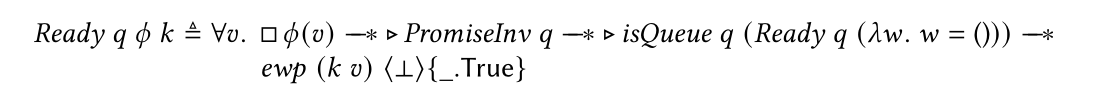
\includegraphics[width=0.75\textwidth]{Hazel_state.png}
\end{figure}
\todo{replace png with latex}

Since our logical state definitions are based on a case study of de Vilhena, we want to give a short comparison of what had to be changed when adapting it to our model of Eio.
First, in the original development the \gsReady{} predicate fulfills two roles.
\begin{enumerate}
  \item It expresses that all continuations in the scheduler's run-queue are safe to execute.
  \item It expresses that all continuations in a promise's waiting-queue are safe to execute.
\end{enumerate}

\gsPInv{} and \gsIsQueue{} were both necessary as preconditions because they are not persistent and need to be passed around explicitly.

In our development \gsPInv{} could be dropped from the definition of Ready because it is now put into an Iris shareable invariant, and can be passed implicitly.
Similarly, the \gsIsQueue{} precondition was dropped from the definition of \gsReady{} because in Eio the run queue must be thread-safe, so the \gsIsQueue{} resource is persistent and can be passed to a fiber once when it is spawned.
Therefore, our \gsReady{} is neither recursive nor mutually recursive with \gsPInv{} anymore, which simplifies its usage in Iris.
We note that the (mutual) recursion was only necessary because \gsPInv{} was used to track global state but was not put into an Iris shareable invariant, so it had to be passed around explicitly in many places.

We also split up the two uses of \gsReady{} and only use it under this name for the first role.
In the case of a scheduler's run-queue, \(Φ\; v\) degenerates just to \(\ulcorner v = () \urcorner\), so we can drop both from the definition and use \(()\) directly.
This is why our definition of \gsReady{} only contains an \ewpt{} without preconditions.

For the second use case of describing the continuations in a promise's waiting-queue we now have another specialized version of \gsReady{}.
As explained in the next section, a broadcast has an invariant \(P\; v \wand \ewp{callback\; ()}{\bot}{\top}\) for all stored \(callback\)s.
This is just \gsReady{} where \(P\; v\) replaces \(Φ\; v\), and it is the same \(P\) as in the definition of the \esuspend{} effect.
